\documentclass{article}
\usepackage{fontspec}
\setsansfont{Helvetica}
\renewcommand{\familydefault}{\sfdefault}
\usepackage{tikz}
\usetikzlibrary{arrows.meta}
\pagestyle{empty}
\definecolor{cA}{HTML}{1F77B4}
\definecolor{cB}{HTML}{FF7F0E}
\definecolor{lookup}{HTML}{2A78D6}
\definecolor{lookuplight}{HTML}{9DC1EC}
\definecolor{write}{HTML}{EB6834}
\definecolor{writelight}{HTML}{F5B597}
\definecolor{ink}{HTML}{0B0B0B}
\definecolor{inktwo}{HTML}{52514E}
\definecolor{gridc}{HTML}{E4E3DF}
\definecolor{axisc}{HTML}{8F8E89}
\definecolor{refc}{HTML}{3D3C39}
\tikzset{
  tick/.style={font=\footnotesize, text=black, inner sep=1.5pt},
  lab/.style={font=\small, text=ink, inner sep=1.5pt},
  note/.style={font=\footnotesize, text=inktwo, inner sep=1.5pt},
  ser/.style={line width=1.4pt, line cap=round, line join=round},
  thin/.style={line width=0.9pt, line cap=round, line join=round},
  ref/.style={line width=0.8pt, draw=refc, dash pattern=on 3pt off 2pt},
}
\begin{document}
\setbox0=\hbox{%
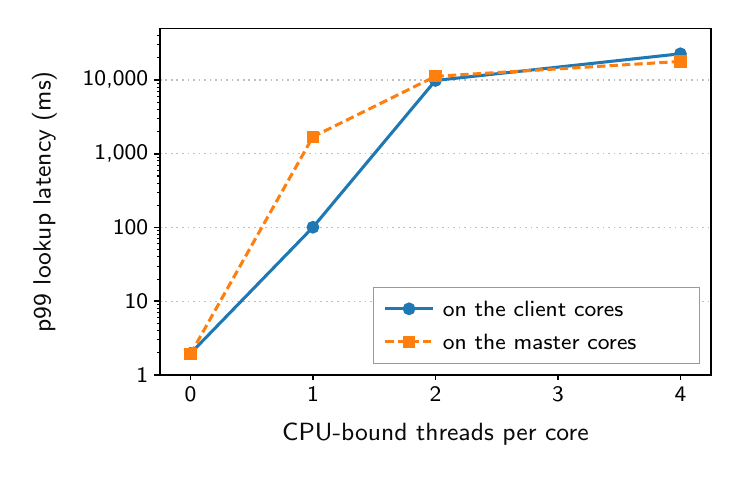
\begin{tikzpicture}[x=1cm,y=1cm]
\draw[black!25, line width=0.4pt, dash pattern=on 0.6pt off 1.4pt] (0.000,0.000) -- (7.000,0.000);
\draw[black, line width=0.6pt] (0.000,0.000) -- (-0.070,0.000);
\node[tick, anchor=east] at (-0.090,0.000) {1};
\draw[black!25, line width=0.4pt, dash pattern=on 0.6pt off 1.4pt] (0.000,0.936) -- (7.000,0.936);
\draw[black, line width=0.6pt] (0.000,0.936) -- (-0.070,0.936);
\node[tick, anchor=east] at (-0.090,0.936) {10};
\draw[black!25, line width=0.4pt, dash pattern=on 0.6pt off 1.4pt] (0.000,1.873) -- (7.000,1.873);
\draw[black, line width=0.6pt] (0.000,1.873) -- (-0.070,1.873);
\node[tick, anchor=east] at (-0.090,1.873) {100};
\draw[black!25, line width=0.4pt, dash pattern=on 0.6pt off 1.4pt] (0.000,2.809) -- (7.000,2.809);
\draw[black, line width=0.6pt] (0.000,2.809) -- (-0.070,2.809);
\node[tick, anchor=east] at (-0.090,2.809) {1,000};
\draw[black!25, line width=0.4pt, dash pattern=on 0.6pt off 1.4pt] (0.000,3.746) -- (7.000,3.746);
\draw[black, line width=0.6pt] (0.000,3.746) -- (-0.070,3.746);
\node[tick, anchor=east] at (-0.090,3.746) {10,000};
\draw[black, line width=0.4pt] (0.000,0.282) -- (-0.040,0.282);
\draw[black, line width=0.4pt] (0.000,0.447) -- (-0.040,0.447);
\draw[black, line width=0.4pt] (0.000,0.564) -- (-0.040,0.564);
\draw[black, line width=0.4pt] (0.000,0.654) -- (-0.040,0.654);
\draw[black, line width=0.4pt] (0.000,0.729) -- (-0.040,0.729);
\draw[black, line width=0.4pt] (0.000,0.791) -- (-0.040,0.791);
\draw[black, line width=0.4pt] (0.000,0.846) -- (-0.040,0.846);
\draw[black, line width=0.4pt] (0.000,0.894) -- (-0.040,0.894);
\draw[black, line width=0.4pt] (0.000,1.218) -- (-0.040,1.218);
\draw[black, line width=0.4pt] (0.000,1.383) -- (-0.040,1.383);
\draw[black, line width=0.4pt] (0.000,1.500) -- (-0.040,1.500);
\draw[black, line width=0.4pt] (0.000,1.591) -- (-0.040,1.591);
\draw[black, line width=0.4pt] (0.000,1.665) -- (-0.040,1.665);
\draw[black, line width=0.4pt] (0.000,1.728) -- (-0.040,1.728);
\draw[black, line width=0.4pt] (0.000,1.782) -- (-0.040,1.782);
\draw[black, line width=0.4pt] (0.000,1.830) -- (-0.040,1.830);
\draw[black, line width=0.4pt] (0.000,2.155) -- (-0.040,2.155);
\draw[black, line width=0.4pt] (0.000,2.320) -- (-0.040,2.320);
\draw[black, line width=0.4pt] (0.000,2.437) -- (-0.040,2.437);
\draw[black, line width=0.4pt] (0.000,2.527) -- (-0.040,2.527);
\draw[black, line width=0.4pt] (0.000,2.601) -- (-0.040,2.601);
\draw[black, line width=0.4pt] (0.000,2.664) -- (-0.040,2.664);
\draw[black, line width=0.4pt] (0.000,2.718) -- (-0.040,2.718);
\draw[black, line width=0.4pt] (0.000,2.766) -- (-0.040,2.766);
\draw[black, line width=0.4pt] (0.000,3.091) -- (-0.040,3.091);
\draw[black, line width=0.4pt] (0.000,3.256) -- (-0.040,3.256);
\draw[black, line width=0.4pt] (0.000,3.373) -- (-0.040,3.373);
\draw[black, line width=0.4pt] (0.000,3.464) -- (-0.040,3.464);
\draw[black, line width=0.4pt] (0.000,3.538) -- (-0.040,3.538);
\draw[black, line width=0.4pt] (0.000,3.600) -- (-0.040,3.600);
\draw[black, line width=0.4pt] (0.000,3.655) -- (-0.040,3.655);
\draw[black, line width=0.4pt] (0.000,3.703) -- (-0.040,3.703);
\draw[black, line width=0.4pt] (0.000,4.027) -- (-0.040,4.027);
\draw[black, line width=0.4pt] (0.000,4.192) -- (-0.040,4.192);
\draw[black, line width=0.4pt] (0.000,4.309) -- (-0.040,4.309);
\draw[black, line width=0.6pt] (0.389,0.000) -- (0.389,-0.070);
\node[tick, anchor=north] at (0.389,-0.090) {0};
\draw[black, line width=0.6pt] (1.944,0.000) -- (1.944,-0.070);
\node[tick, anchor=north] at (1.944,-0.090) {1};
\draw[black, line width=0.6pt] (3.500,0.000) -- (3.500,-0.070);
\node[tick, anchor=north] at (3.500,-0.090) {2};
\draw[black, line width=0.6pt] (5.056,0.000) -- (5.056,-0.070);
\node[tick, anchor=north] at (5.056,-0.090) {3};
\draw[black, line width=0.6pt] (6.611,0.000) -- (6.611,-0.070);
\node[tick, anchor=north] at (6.611,-0.090) {4};
\draw[line width=1.1pt, line join=round, draw=cA] (0.389,0.273) -- (1.944,1.876) -- (3.500,3.740) -- (6.611,4.079);
\draw[line width=1.1pt, line join=round, draw=cB, dash pattern=on 3pt off 1.5pt] (0.389,0.266) -- (1.944,3.025) -- (3.500,3.793) -- (6.611,3.982);
\filldraw[fill=cA, draw=cA, line width=0.8pt] (0.389,0.273) circle (1.9pt);
\filldraw[fill=cA, draw=cA, line width=0.8pt] (1.944,1.876) circle (1.9pt);
\filldraw[fill=cA, draw=cA, line width=0.8pt] (3.500,3.740) circle (1.9pt);
\filldraw[fill=cA, draw=cA, line width=0.8pt] (6.611,4.079) circle (1.9pt);
\filldraw[fill=cB, draw=cB, line width=0.8pt] (0.389,0.266) +(-1.8pt,-1.8pt) rectangle +(1.8pt,1.8pt);
\filldraw[fill=cB, draw=cB, line width=0.8pt] (1.944,3.025) +(-1.8pt,-1.8pt) rectangle +(1.8pt,1.8pt);
\filldraw[fill=cB, draw=cB, line width=0.8pt] (3.500,3.793) +(-1.8pt,-1.8pt) rectangle +(1.8pt,1.8pt);
\filldraw[fill=cB, draw=cB, line width=0.8pt] (6.611,3.982) +(-1.8pt,-1.8pt) rectangle +(1.8pt,1.8pt);
\draw[black, line width=0.6pt] (0.000,0.000) rectangle (7.000,4.400);
\node[lab, anchor=north] at (3.500,-0.550) {CPU-bound threads per core};
\node[lab, rotate=90, anchor=south] at (-1.250,2.200) {p99 lookup latency (ms)};
\draw[fill=white, draw=black!40, line width=0.4pt] (2.715,1.110) rectangle (6.850,0.150);
\draw[line width=1.1pt, line join=round, draw=cA] (2.865,0.840) -- (3.465,0.840);
\filldraw[fill=cA, draw=cA, line width=0.8pt] (3.165,0.840) circle (1.9pt);
\node[tick, anchor=west] at (3.535,0.840) {on the client cores};
\draw[line width=1.1pt, line join=round, draw=cB, dash pattern=on 3pt off 1.5pt] (2.865,0.420) -- (3.465,0.420);
\filldraw[fill=cB, draw=cB, line width=0.8pt] (3.165,0.420) +(-1.8pt,-1.8pt) rectangle +(1.8pt,1.8pt);
\node[tick, anchor=west] at (3.535,0.420) {on the master cores};
\end{tikzpicture}}%
\pdfvariable horigin=0pt
\pdfvariable vorigin=0pt
\pagewidth=\dimexpr\wd0+8pt\relax
\pageheight=\dimexpr\ht0+\dp0+8pt\relax
\shipout\vbox{\kern4pt\hbox{\kern4pt\box0\kern4pt}\kern4pt}
\end{document}
